\documentclass{report}
\usepackage[french,english]{babel}
\usepackage{geometry}
 \geometry{
 a4paper,
 total={150mm,245mm},
 left=30mm,
 top=25mm,
 }
\usepackage{hyperref}
\usepackage[nodayofweek,level]{datetime}
\usepackage[utf8]{inputenc}
\usepackage[T1]{fontenc}
\usepackage[toc,page]{appendix}
\usepackage{float}
\usepackage{import}
\usepackage{amsmath} 
\usepackage[]{graphics}
\usepackage{graphicx}
\usepackage{caption}
\usepackage{subcaption}
\usepackage[usenames, dvipsnames]{color}
\usepackage{lipsum}
\usepackage{fancyhdr}
\usepackage{pdfpages}

\graphicspath{ {images/} }

\begin{document}
\selectlanguage{english}
\pagenumbering{gobble}
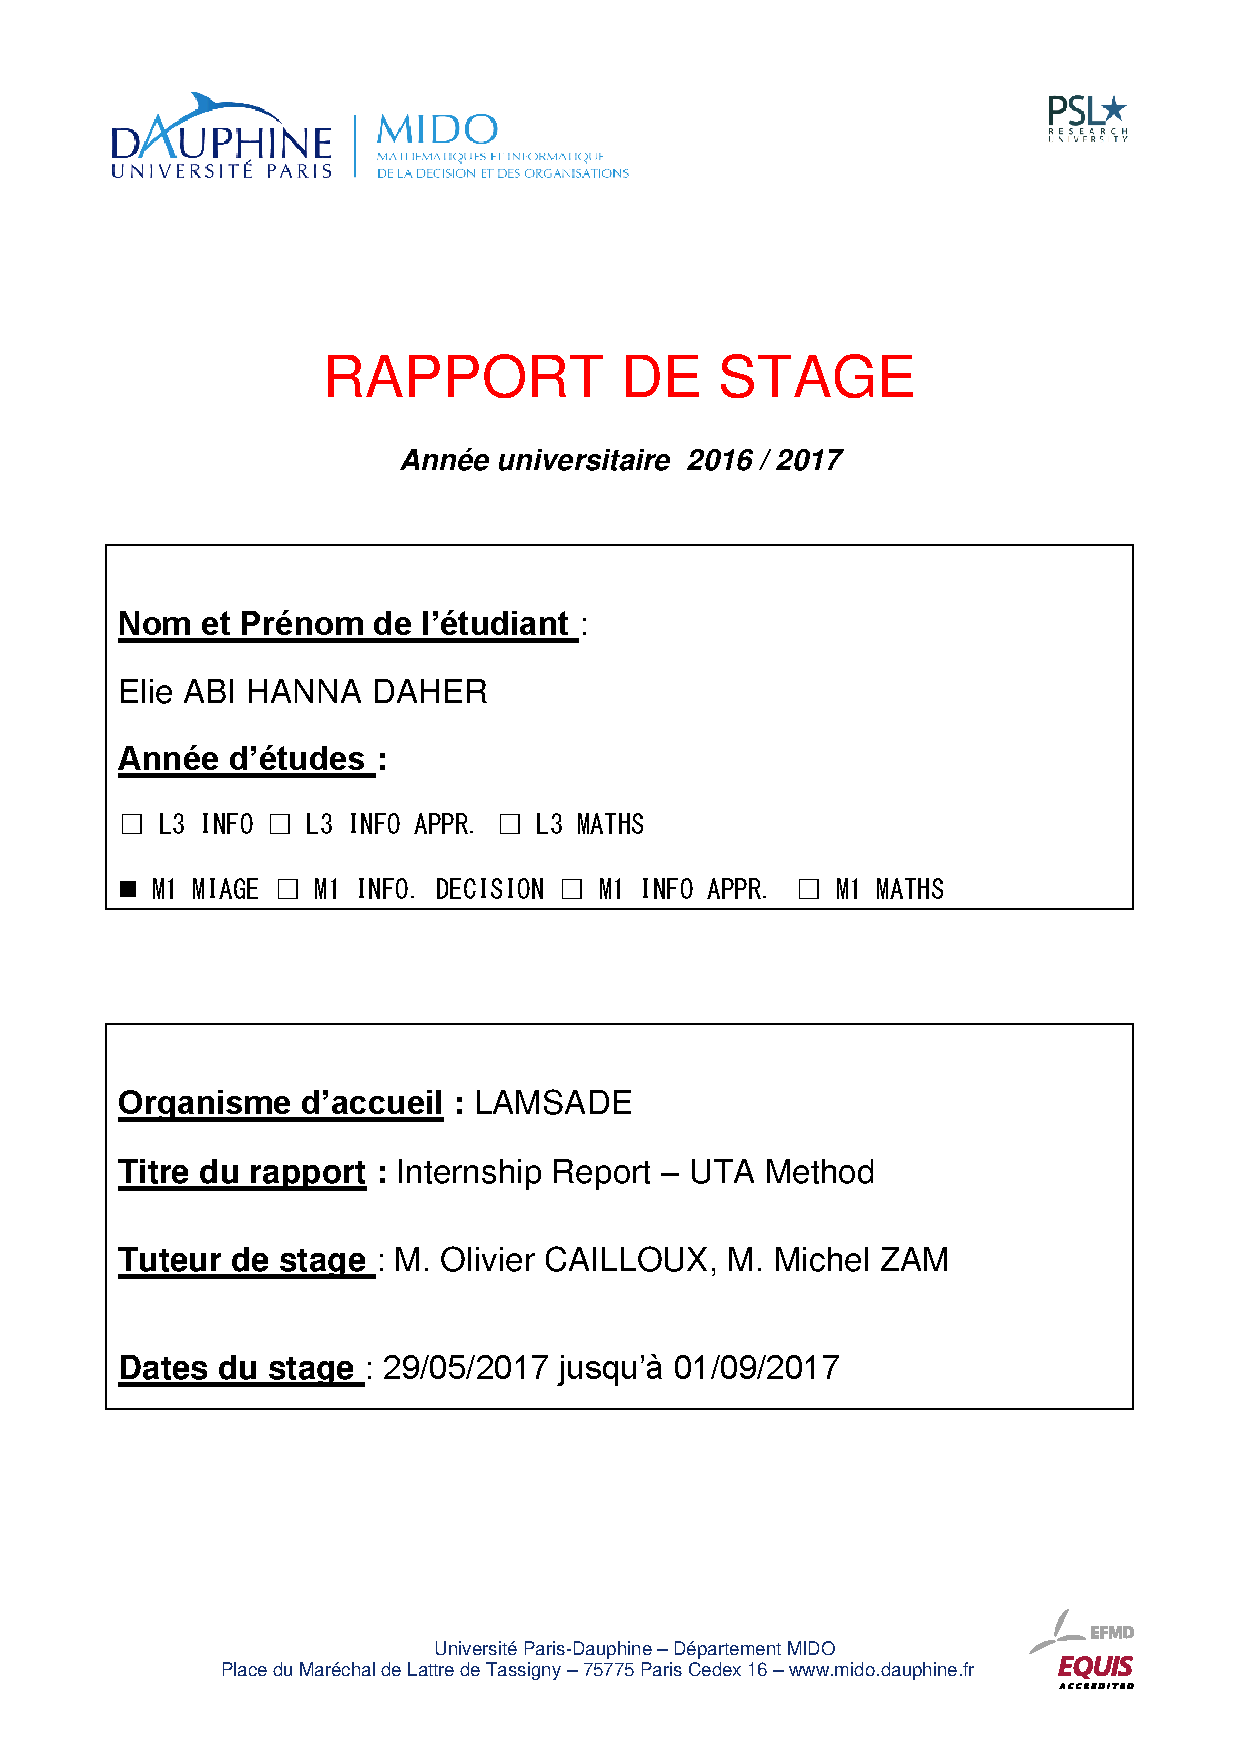
\includepdf{cover-page.pdf}

\begin{titlepage}

\newcommand{\HRule}{\rule{\linewidth}{0.5mm}}
\center

\textsc{\LARGE LAMSADE}\\[1.5cm] 
\textsc{\Large M1 MIAGE}\\[0.5cm]
\textsc{\large Internship}\\[0.5cm] 

\HRule \\[0.4cm]
{ \huge \bfseries Internship Report - UTA Method} 
\HRule \\[1.5cm]

\begin{minipage}{0.4\textwidth}
\begin{flushleft} \large
\emph{Student:}\\
Elie \textsc{Abi Hanna Daher}\\ 
\textcolor{white}{blank space}
\end{flushleft}
\end{minipage}
~
\begin{minipage}{0.4\textwidth}
\begin{flushright} \large
\emph{Supervisor:} \\
M. Olivier \textsc{Cailloux} \\
M. Michel \textsc{Zam} 
\end{flushright}
\end{minipage}\\[2cm]

\newcommand{\mydate}{\formatdate{25}{8}{2017}}
{\large \mydate}\\[2cm] 

\begin{figure}[h]
\makebox[\textwidth]{

\includegraphics[width=0.40\textwidth]{dauphine.png}
\hfill    

\includegraphics[width=0.40\textwidth]{lamsade.png}
}\\[0.5cm]
\end{figure}

\vfill

\end{titlepage}

\abstract 
This report documents the work done during the summer internship at LAMSADE Dauphine, under the supervision of Mr. Olivier Cailloux and Mr. Michel Zam. The report give an overview of the projects completed during the internship.\\
I have worked mainly on the UTA method which is an ordinal regression method, proposed by E. Jacquete-Lagreze and J. Siskos, which adjust a system of additive utility function.
\newpage
{ \huge \bfseries Acknowledgment}\\[0.3cm]
\\

There are a number of people that I would like to thank them for their help and contribution in the success of my internship at LAMSADE Dauphine.\\

First and foremost, I would like to thank Mr. Olivier Cailloux, a lecturer in computer science and researcher at LAMSADE. His advice and follow ups helped me a lot in establishing my assignments during the internship.\\

I also would like to thank Mr. Michel Zam, the founder of KarmicSoft and an associate professor at Paris Dauphine University, for the opportunity given to me as an intern at Lamsade\\

Doing my internship at LAMSADE with Mr. Cailloux and Mr. Zam was a pleasure, I have learned a lot thanks to them. I would like to them for this opportunity.\\

I would like to thank the internship manager, Mrs Maude Manouvrier, for all her efforts in term of follow-up as well as her availability and patience to answer my questions.\\
\newpage
\tableofcontents{}
\newpage
\pagenumbering{arabic}

\chapter{Introduction}
Currently I'm completing my master's degree in MIAGE at Paris Dauphine University so I had the opportunity to achieve an internship at LAMSADE (Laboratoire d'analyse et modélisation de systèmes pour l'aide à la décision). LAMSADE is a Paris-Dauphine research laboratory specialized in decision theoretic approaches. Decision theory aims at helping individuals who face decision problem by elaborating a study of the reasoning underlying agent's choices. \\

From \formatdate{29}{5}{2017} to \formatdate{1}{9}{2017}, I completed a research internship at LAMSADE at Paris Dauphine University. My internship was made remotely, so I had a weekly meeting with Mr. Cailloux to get feedback of the work done. And I communicated with Mr. Zam via mails or calls. \\

This internship was very important for my professional career because it may be my last internship before I get my Masters's degree in Information systems for finance at Paris Dauphine University. Let's not also forget that this internship will allow me to practice the different courses learned throughout my academic years.\\

One of the objectives is to propose the UTA method, that solve a multi-criteria problem by building a utility function based on the preferences of the Decision Maker, as an open source software component. Another objective was to integrate this open source software into DecisionCloud, a software based on MyDraft a tool developed by KarmicSoft a LAMSADE spin-off. Researching similar literature and research represent an important objective in this internship. \\

In this internship report, I will describe the context of the project which contains an overview of the internship. Writing this reports, I will describe the projects made: UTA, LinearProgram Solver, UTA Calculator and the research realized. I will conclude by reflecting on the flow of the internship. \\

\chapter{Context of the projects}
\section{Introduction to LAMSADE}
LAMSADE is a laboratory located in Paris Dauphine university. Lamsade stands for Laboratoire d'analyse et modélisation de systèmes pour l'aide à la décision. The french laboratory has been established in 1974 by Bernard Roy. The main research subjects that this center study are  operational research, decision aid, artificial intelligence (AI) and decision theory. \\
The activities of LAMSADE are divided into 3 poles: 
\begin{itemize}
\item Decision aid 
\item Combinatorial optimization and algorithmic
\item Data Science
\end{itemize}
LAMSADE is well know for the origin of the multiple-criteria decision analysis (MCDA), and for its approach to the Algorithmic Decision Theory. The laboratory has established himself between the best internationally. \\
LAMSADE is structured in 2 dimensions:
\begin{itemize}
\item Scientific 
\item Research
\end{itemize}
Scientific dimension represent the poles, where there is a community of researches invited to exchange through out meetings and seminary. The research dimension represent the projects assembled by the researches interested in the subject in question. Both of this dimensions are neither fixed neither permanent, they can be submitted to an evaluation by the Laboratory. 

\section{Objectives}
Through out the internship, I had several objectives to achieve and those objectives changed from when we began the internship. \\
The following list represent the objectives stated at the beginning of the internship: 
\begin{itemize}
\item Propose an open source software component of the UTA method (Main objective)
\item Integrate the UTA open software component as one of the tools in the Decision Deck community
\item Document and publish the software and implement a graphical user interface to the UTA by using DecisionCloud, a tool promoted by the Decision Deck
\end{itemize}

So as stated before, the objectives changes from the beginning of the internship for different reasons. We ended up doing an open source software component of the UTA method and we published on github instead of the DecisionCloud. This gave us the opportunity to develop more the software by doing more functionalities, and allowed us to specify time for research. So the main reason that we weren't being able to make the tools in the Decision Deck community because Mr. Zam wasn't available to assist me. So we took this opportunity to make the software more developed.\\
So during the internship the objectives were re-stated as follow: 
\begin{itemize}
\item Summarize UTA
\item Propose an open source software component of the UTA method
\item Generate Random alternatives and criteria
\item Generate Value Function
\item Search literature for existing similar studies, and how to generate realistic random alternatives
\end{itemize}

\section{Conduct of the internship}
The \formatdate{29}{5}{2017} I started my internship. The first two weeks, was dedicated to get to know the platform MyDraft and create some basic applications. MyDraft is a platform created by KarmicSoft, it specialized in building and running data-driven Web applications. It is a platform for developing business application the easiest way without complexity. During the two weeks, I did all the tutorials available in the site and in addition I created my own project. The project was called \textit{StockApp} where I recreated a project done during the course of \textit{Marché Financier}: Portfolio Management Project. The project consist in collecting stock information and calculating the following information: 
\begin{itemize}
\item Weekly Returns of assets by calculating its mean and standard deviation. 
\item Correlation matrix of the stock returns
\item Correlation of stock returns with the stock market index
\item Beta, Sharpe Ratio and Treynor Ratio
\item Portfolio optimization scheme of Markowitz
\end{itemize}
I succeed in doing most of the functionalities of the project but the last point wasn't possible to do in MyDraft since it needed the Macro used in the Excel.\\

After learning about the platform MyDraft, I had a meeting with Mr. Cailloux the \formatdate{15}{6}{2017} where he introduced me a little bit about the UTA method and gave me the book: \textit{Multiple Criteria Decision Analysis}, where the chapter 9 contains an explication about the UTA method. I had to understand this method and make a summary about it, so I took this opportunity to learn about LaTeX to create the summary using LaTeX. Till the end of the month of July, we created the summary of UTA method in Latex, and created my own problem to illustrate the method. Since one of the step of the method was to solve a Linear Program, so we created an independent project to solve a simple Linear Program (LP) by using  the google ortools (Optimization tools) library. During that time I made some research about literature for existing similar studies, and how to generate realistic random alternatives research. During this time we had a weekly meeting with Mr. Cailloux.\\

At the end of the month of July, we had a meeting Mr. Cailloux and me to discuss about the software that will represent the UTA method. We designed the architecture, and I coded the program, I didn't took long because during the month before I had already worked on little components of the software. During the month of august our goal was to finish this document and to make simulation and testing the software.\\  

All of the work done is available as open source on my github repository: \url{ https://github.com/elieahd/decision-uta-method}.\\

So in the next chapter, we will discuss the projects done above, without including the part of MyDraft since we didn't use it in our project due to the change of objectives. 

\chapter{Description of the projects}
\section{UTA}
\subsection{Introduction of the aid decision}
In decision theory we elaborate a study of reasoning underlying the agent choices. Two branches can be broken from the decision theory: giving an advice on how to make the best decisions, or how existing agents actually make decisions. \\
In multiple-criteria decision analysis (MCDA), the following concepts play a fundamental role in decision-making problems: 
\begin{enumerate}
\item object of the decision, definition of the set of potential actions(alternatives) and the determination of a problem statement
\item modeling a consistent family of criteria
\item defining a global preference model
\item decision-aid or decision support
\end{enumerate}

\underline{Example: Buying a new car} \\
Let's consider we are trying to figure out which car to buy. Using the methodology represented above, we state that the objective of this problem is \textbf{buying a new car}. After stating the objective, we can list the potential of actions that represent the list of cars that we may buy. By potential action, we designate that which constitutes the object of the decision. An action is qualified as potential when it is deemed possible to implement it or if it has some interest within the decision aiding process. So the following list represent the potential actions of this example: 
\begin{itemize}
\item Peugeot 208 GTi
\item Nissan Sentra
\item Citroen C4
\item Peugeot 308 berline
\end{itemize}
After listing the list of potential cars, we can define a list of criteria that we will base our decision on. A criterion is constructed to evaluate and compare potential actions according to a point of view. So when defining the list of criteria you should always remember that they must be easy to evaluate (easy to convert to a scale) and should be logical.
Let's say we will base our purchase on the following criteria:
\begin{itemize}
\item price (in Euro)
\item comfort (0, +, ++, +++) \textit{0 being not comfortable and +++ very comfortable}
\item safety (1, 2, 3, 4, 5) \textit{1 being not safety and 5 safe}
\end{itemize}
During the decision process, we will determinate the global preferences of the potential actions:
\begin{enumerate}
\item Citroen C4
\item Peugeot 208 GTi
\item Peugeot 308 berline
\item Nissan Sentra
\end{enumerate}
Once the global preference is defined, we can start the decision support.\\

One of the multi-criteria decision analysis methods is the UTA method, which was proposed by E. Jacquet-Lagrèze and J. Siskos in 1982. This method is proposed by the Multi-Attribute Utility Theory (MAUT) that build a utility function based on the DM\footnote{Decision Maker} preferences.\\ 

The UTA method is used to solve a multi-criteria problem by building a utility function based on the preferences of the DM and solving a linear program (LP). It adopt the aggregation-disaggregation principles: where the model is based on a given preferences.\\ The UTASTAR, a variant of the UTA method, has been considered a better algorithm than UTA. Better result were found using the UTASTAR algorithm. So this is why we will focus on this method rather than the UTA method.\\The aim of the UTASTAR method is to estimate a set of additive utility functions which are as consistent as possible with the decision maker's preferences.\\
At the beginning of the problem, the DM should present the following information 
\begin{itemize}
\item rank of the actions
\item give the criteria he want to base his decision on 
\item evaluate the action compared to the criterion
\end{itemize}
Once those information are presented, the UTASTAR algorithm can be executed. 

\newpage
\subsection{Principles and Notation}
Let's call $A={a,b,c,...}$ the set of potential actions and $g_1, g_2, g_3, ..., g_n$ the family of criteria. Where $g_i(a)$ represent the funtion of an action(alternative)$a$ on the criteria $g_i$ with $a \in A_R$. \\

We define $g_{i*}$ as the least preferred criteria: $g_{i*} = min_{a \in A} g_i (a)$ and $g_i^{*}$ as the most preferred criteria: $g_i^{*} = max_{a \in A} g_i (a)$. So the interval for each criteria $g_i$ is: $[g_{i*} , g_i^{*}]$.\\

If we want to evaluate two actions, for example $a$ and $b$, on only one criteria $g_i$ we have the following relations: 
\begin{equation}
      \begin{cases}
      	a \succ b\Leftrightarrow g_i(a) > g_i(b) \quad preference\\
      	a\sim b \Leftrightarrow g_i(a) = g_i(b) \quad indifference \\
      \end{cases}
\end{equation}
The criteria aggregation model in UTASTAR has the following form:
\begin{equation}\label{eq1}
      v(g(a)) = \sum_{i=1}^{n} v_i (g_i (a))
\end{equation}
subject to normalization constraints:\\
\begin{equation}\label{eq2}
      \begin{cases}
      	\sum_{i=1}^{n} v_i(g_{i}^{*}) = 1\\
       	v_i(g_{i*})= v_i(g_i^1)  = 0,  \forall i = 1, 2, ..., n\\
      \end{cases}
\end{equation}
where $ v_i, i = 1,2,...,n$ are non decreasing real valued function.\\
In UTASTAR we have 
\begin{equation}
	w_{ij} = v_i(g_i^{j+1}) - v_i(g_i^{j}) \geq 0 \quad \forall i \quad j 
\end{equation}
Which will allow us to write: 
\begin{equation}
	v_i(g_i^j) =	  \sum_{t=1}^{j-1} w_{it} \quad \forall i = 1,2,...,n \quad and \quad j = 2,3,...,\alpha _i -1 \\
\end{equation}
With the evaluation of an action a $g(a) = [g_1(a) ,  g_2(a) , ... , g_n(a)] $, we have the following relation:
\begin{equation}
      \begin{cases}
      	v[g(a)] > v[g(b)] \Leftrightarrow a \succ b\\
      	v[g(a)] \sim v[g(b)] \Leftrightarrow a = b\\
      \end{cases}
\end{equation}

\newpage
\subsection{Development} 
The updated version of UTA, UTASTAR, propose a double error function for each action: $\sigma ^{+} (a)$ and $\sigma ^{-} (a)$.  So the value of each alternative $a \in A_R$ can be written: \\
\begin{equation}
	v^{'} [g(a)] = \sum_{i=1}^{n} v_i [g_i (a)] - \sigma ^{+} (a)+ \sigma ^{-} (a) \quad  \forall a \in A_R
\end{equation}
\begin{figure}[H]
    	\centering
	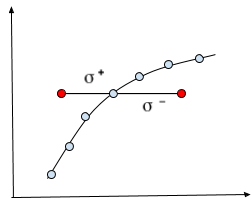
\includegraphics{error-function-utastar}
	\caption{Error function in UTASTAR}
\end{figure}
For each criteria, the interval $[g_{i*}, g_i^{*}]$ is cut into $(\alpha _i -1)$ equals interval, and the end points $g_i^{j}$ are given by the formula:
\begin{equation}
	g_i^{j}= g_{i*} + \frac{j-1}{\alpha _i -1} (g_i^{*} - g_{i*})  \forall j = 1,2, ..., \alpha _i
\end{equation}
The marginal value of an action $a$ is calculated by a linear interpolation
\begin{equation}
	v_i [g_i (a)] = v_i (g_i^{j}) + \frac{g_i (a) - g_i^{j}}{ g_i^{j+1} - g_i^{j}} [v_i (g_i^{j+1}) - v_i (g_i^{j}) ] 
\end{equation}
The set of reference action $ A_R = a_1, a_2, ... , a_m$ is arranged where $a_1$ is the best action and $a_m$ is the worst action. Which indicate that we have two possible situations:
\begin{itemize}
\item $a_k  \succ a_{k+1} \quad $ preference 
\item $a_k \sim a_{k+1} \quad $ indifference
\end{itemize} 
So if we have that $\Delta (a_k, a_{k+1} ) = v^{'} [g(a_k)] - v^{'} [g(a_{k+1})]$ and $\delta$ is a small positive number we will obtain the following relations: 
\begin{equation}\label{eq3}
      \begin{cases}
      	\Delta (a_k, a_{k+1} ) \geq \delta\\
       	\Delta (a_k, a_{k+1} ) = 0 \\
      \end{cases}
\end{equation}
The marginal value functions are estimated by means of the Linear Programm with \eqref{eq1}, \eqref{eq2}, \eqref{eq3} as constraints, and an objective function depending on the $ \sigma^{+}$ and $\sigma^{-} $: 
$$ [min]z = \sum_{k=1}^{m} [ \sigma ^{+} (a_k) + \sigma ^{-} (a_k)]  $$
subject to: 
\begin{equation}\label{eq5}
      \begin{cases}
      	\Delta (a_k, a_{k+1} ) \geq \delta \quad or \quad \Delta (a_k, a_{k+1} ) = 0 \\
      	\sum_{i=1}^{n} \sum_{j=1}^{\alpha_i -1} w_{ij} = 1\\
       	w_{ij} \geq 0, \quad \sigma^{+}(a_k) \geq 0, \quad \sigma^{-}(a_k) \geq 0, \quad  \forall i, j  and  k\\
      \end{cases}
\end{equation}

\subsection{Example - Buying New Car}
The implementation of UTASTAR algorithm is illustrated by an example I made: \textbf{buying a new car}. Another example is available in the Appendices, Choice of transportation, this example was taken from the book: Multiple Criteria Decision Analysis.\\ The DM is interested only in the following criteria:
\begin{itemize}
\item price (in Euro)
\item comfort ($0$, +, ++, +++) \textit{0 being not comfortable and +++ very comfortable}
\item safety ($1, 2, 3, 4, 5$) \textit{1 being not safety and 5 safe}
\end{itemize}
The evaluation of the previous criteria is presented in the following table: 
\begin{center}
 \begin{tabular}{|c | c c c c|} 
 \hline
 Cars & Price & Comfort & Safety & Ranking of the DM \\ [0.5ex] 
 \hline
 Nissan Sentra (ns) & 17\,000 & +++ & 4 & 1 \\ 
 \hline
 Citroen C4 (c4) & 15\,000& ++ & 2 & 2\\ 
 \hline
 Peugeot 208 GT (p208) & 25\,000 & + & 3 & 3\\
 \hline
 Peugeot 308 berline (p308)& 18\,500 & 0 & 3 & 4\\
 \hline
\end{tabular}
\end{center}
First of all, we should specify the scale \footnote{the interval $[g_{i*}, g_{i}^{*}]$ is cut into equal intervals} for each criteria.
\begin{itemize}
\item Price $\quad \Rightarrow \quad [g_{1*}, g_{1}^{*}] = [25\,000, 20\,000, 15\,000]$
\item Comfort $\quad \Rightarrow \quad [g_{2*}, g_{2}^{*}] = [0, +, ++, +++]$
\item Safety $\quad \Rightarrow \quad [g_{3*}, g_{3}^{*}] = [1, 3, 5]$
\end{itemize}
According to this formula: $v(g(a)) = \sum_{i=1}^{n} v_i (g_i (a))$ , the value of each alternative may be written: 
\begin{itemize}
\item $v(g(ns)) =  0.4v_1(15\,000) +  0.6v_1(20\,000) + v_2(+++) + 0.5v_3(3) + 0.5v_3(5)  $
\item $v(g(c4)) = v_1(15\,000) + v_2(++) + 0.5 v_3(1) + 0.5v_3(3) = v_1(15\,000) + v_2(++) + 0.5v_3(3)$
\item $v(g(p208)) = v_1(25\,000) + v_2(+) + v_3(3) = v_2(+) + v_3(3) $
\item $v(g(p308)) = 0.3v_1(15\,000) +  0.7v_1(20\,000) + v_2(0) + v_3(3) = 0.3v_1(15\,000) +  0.7v_1(20\,000) + v_3(3)$
\end{itemize}
We have that $v_1(25\,000) = v_2(0) = v_3(1) = 0$. \\
Since the marginal value $v_i(g_i)$ can be expressed in terms of variables $w_{ij}$: $v_i(g_i^{j}) = \sum _{t=1}^{j-1} w_{it}$ , the value of each alternative can be written: 
\begin{itemize}
\item $v(g(ns)) = w_{11} + 0.4w_{12} + w_{21} + w_{22} + w_{23} + w_{31} + 0.5w_{32}$
\item $v(g(c4)) = w_{11} + w_{12} + w_{21} + w_{22} + 0.5w_{31}$
\item $v(g(p208)) = w_{21} + w_{31} $
\item $v(g(p308)) = w_{11} + 0.3w_{12} + w_{31}$
\end{itemize}
For each pair of consecutive alternatives, we express the difference between them: 
\begin{itemize}
\item $\Delta (ns,c4) =  -0.6w_{12} + w_{23} + 0.5w_{31} +  0.5w_{32}  -\sigma _{ns}^{+} +\sigma _{ns}^{-} +\sigma _{c4}^{+} - \sigma _{c4}^{-} $
\item $\Delta (c4, p208) = w_{11} + w_{12} + w_{22} - 0.5w_{31} -\sigma _{c4}^{+} +\sigma _{c4}^{-} +\sigma _{p208}^{+} - \sigma _{p208}^{-} $
\item $\Delta (p208, p308) =w_{21} - w_{11} - 0.3w_{12} -\sigma _{p208}^{+} +\sigma _{p208}^{-} +\sigma _{p308}^{+} - \sigma _{p308}^{-} $
\end{itemize}
Having $\delta = 0.05$, we can solve the following LP:\\

Objective:  
\begin{equation}
	Minimize \quad \sum_{a \in A} \sigma _{a}^{+} + \sigma _{a}^{-}
\end{equation}

Subject to: \\
\begin{equation}
	\begin{cases}
		 -0.6w_{12} + w_{23} + 0.5w_{31} + 0.5w_{32}  -\sigma _{ns}^{+} +\sigma _{ns}^{-} +\sigma _{c4}^{+} - \sigma _{c4}^{-}   \geq 0.05\\
		 w_{11} + w_{12} + w_{22} - 0.5w_{31} -\sigma _{c4}^{+} +\sigma _{c4}^{-} +\sigma _{p208}^{+} - \sigma _{p208}^{-} \geq 0.05 \\
		w_{21} - w_{11} - 0.3w_{12} -\sigma _{p208}^{+} +\sigma _{p208}^{-} +\sigma _{p308}^{+} - \sigma _{p308}^{-}  \geq 0.05 \\
		w_{11} + w_{12} + w_{21} + w_{22} + w_{23} + w_{31} + w_{32} = 1
	\end{cases}
\end{equation}
An optimal solution is $w_{12} = 0.34$, $w_{21} = 0.152$, $w_{32} = 0.51$ with $\sum_{a \in A} \sigma _{a}^{+} + \sigma _{a}^{-} = 0$. The utilities found for each alternative are as follows: \\ 
\begin{itemize}
\item $v(g(ns)) = 0.543$
\item $v(g(c4)) = 0.492$
\item $v(g(p208)) = 0.152 $
\item $v(g(p308)) = 0.102 $
\end{itemize}
Those utilities are consistent with the DM's preference ranking. \\

The UTA method build a utility function based on the preferences of the DM and it consist in solving a linear program (LP) to solve a multi-criteria problem.\\
This method will elaborate a model of preferences which is as similiar as possible to the DM's preferences.\\
The improved version of the UTA, UTASTAR, has performed better than the regular method.

\section{Linear Program Solver}
One of the steps of the UTA algorithm is solving the Linear Program. So we can complete the UTA algorithm, I created an independant java application that has the objectif of solving the LP by finding the optimal solution.\\
So i can achieve this goal I had to use the google ortools (Optimization tools) library. You can find those library in the github repository under src/libs.
\begin{figure}[H]
    	\centering
	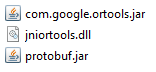
\includegraphics[width=4cm,height=1.5cm,keepaspectratio]{lp-libs.png}
	\caption{Library used in the solver}
\end{figure}
Let's talk the following example:\\

Objective:  
\begin{equation}
Maximize \quad 10x_1 + 6x_2 + 4x_3
\end{equation}

subject to: \\
\begin{equation}
	\begin{cases}
		x_1 + x_2 + x_3 \leq 100\\
		10x_1 + 4x_2 + 5x_3 \leq 600\\
		2x_1 + 2x_2 + 6x_3 \leq 300\\
	\end{cases}
\end{equation}
So we can solve the LP, we need to create an instance of the solver:
\begin{figure}[H]
    	\centering
	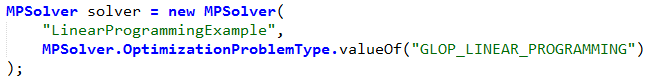
\includegraphics[width=\textwidth]{lp-solver.png}
	\caption{Java code to define the solver}
\end{figure}
After that, we define the 3 variables $x_1$, $x_2$ et $x_3 \quad  \in \quad [0 ; \infty]$: \\
\begin{figure}[H]
    	\centering
	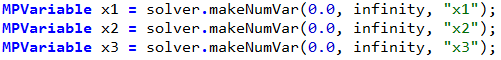
\includegraphics[width=10cm,height=3cm,keepaspectratio]{lp-variables.png}
	\caption{Java code to define the variables of the LP}
\end{figure}
We define the objective $Maximize \quad 10x_1 + 6x_2 + 4x_3$: \\
\begin{figure}[H]
    	\centering
	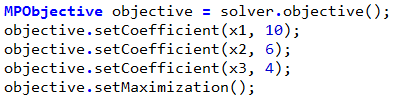
\includegraphics[width=8cm,height=2cm,keepaspectratio]{lp-objectif.png}
	\caption{Java code to define the objective of LP}
\end{figure}
We do the same for the constraint: \\
\begin{figure}[H]
    	\centering
	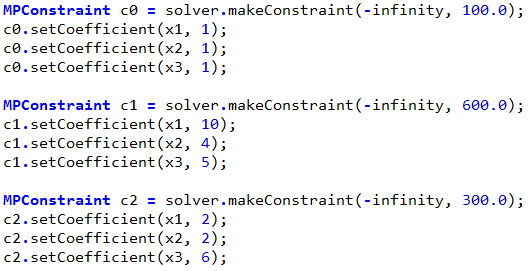
\includegraphics[width=10cm,height=6cm,keepaspectratio]{lp-constraints.png}
	\caption{Java code to define the constraints of the LP}
\end{figure}
After setting all the constraints and variables we can execute the solver: \\
\begin{figure}[H]
    	\centering
	
\includegraphics[width=10cm,height=6cm,keepaspectratio]{lp-solve.png}
	\caption{Java code for running the solver}
\end{figure}
After executing the solver, we display the optimal value of the objective and the value of the variables: \\
\begin{figure}[H]
    	\centering
	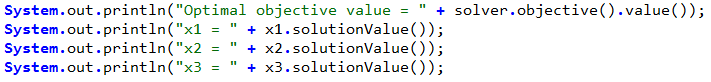
\includegraphics[width=\textwidth]{lp-result.png}
	\caption{Java code for displaying the result of the solver}
\end{figure}
Once you run the program, you will have the following the result: 
\begin{center}
Optimal objective value = 733.3333333333\\
x1 = 33.33333333336\\
x2 = 66.66666666666\\
x3 = 0.0\\
\end{center}

\section{Research}
One aspect of this internship is the research. The objective of the research was to find similar studies, how to generate realistic random alternatives and studies made on UTA method.
\subsection{Comparative analysis of UTA multicriteria methods}
This paper written by Michel Beuthe and Giuseppe Scannella and it is mainly about the variants of UTA method. As discussed in this paper a method of multi-criteria analysis is chosen depending on the circumstances of the decision making.UTA makes possible the estimation of a nonlinear additive function, which is obtained by the use of a linear program and the only information required from the decision maker are the global preferences between projects. \\
After the execution of the algorithm we should always be possible to converse with the decision maker in order to specify the precision of the preferences stated\\
The value $\delta$ must not be given too high an initial value. In the basic model, it was noted that the values given to $\delta$ were to some extent arbitrary. 
\subsubsection{Simulations}
The simulation are applied to the case of 353 road projects in Belgian Network during the period 1985-2010. The Center of Road Research (CRR) realized a multi criteria analysis  that used 29 criteria regrouped in six main themes: 
\begin{itemize}
\item safety on the present road
\item projects socioeconomic aspects
\item impact on environment
\item current and future traffic
\item problems of planning and urbanism
\item wear state of the current road.
\end{itemize}
The 29 criteria has been established with a scale going from 1 to 5. 

\subsubsection{Variants of UTA}
\begin{enumerate}
\item UTA
\item UTASTAR
\item UTA2
\item UTAMKEN
\item UTAMP1
\item UTAMP2
\item UTAMIME
\item UTASTARMIME
\item UTA2MIME
\end{enumerate}

\subsubsection{Conclusions made}
When there is no error in the utility function estimation, $ \sum_{a \in A} \sigma _{a}^{+} + \sigma _{a}^{-} = 0$, the basic UTA method provides the most practical and efficient method of estimation. \\
Even when there is interdependence between criteria, the UTA approach provides good results. \\
In the case where the utility function estimation is positive, $ \sum_{a \in A} \sigma _{a}^{+} + \sigma _{a}^{-} >0 0$, the UTASTAR appears more reliable.\\
The simulations results indicate that small value of $\delta$  lead to better results in case of a positive utility function estimation. But in case of no error in the utility function estimation, larger value of $\delta$ can provide better results. The use of UTAMP1 or UTAMP2 may then be used to find the practical upper bound of the values given.  

\subsection{Disadvantages of the UTA method}
\begin{enumerate}
\item We can always question the decision marker about his preferences
\item Solution may not be the only one as in any LP we can have different solutions
\end{enumerate}

\newpage
\section{Implementation - UTA Calculator}
We wanted to implement the UTASTAR method. In order to make it possible we created this java program: AlternativeCriteria. So basically we will generate a decision problem and run the UTASTAR algorithm. \\
Another objective we were trying to achieve was to generate random alternatives and criteria, so we can generate a decision problem. \\
After solving the problem our goal was to get the $v^{R}$ and $v^{T}$ and compare them. 
\subsection{Architecture}
\subsubsection{Class Diagram}
\begin{figure}[H]
    	\centering
	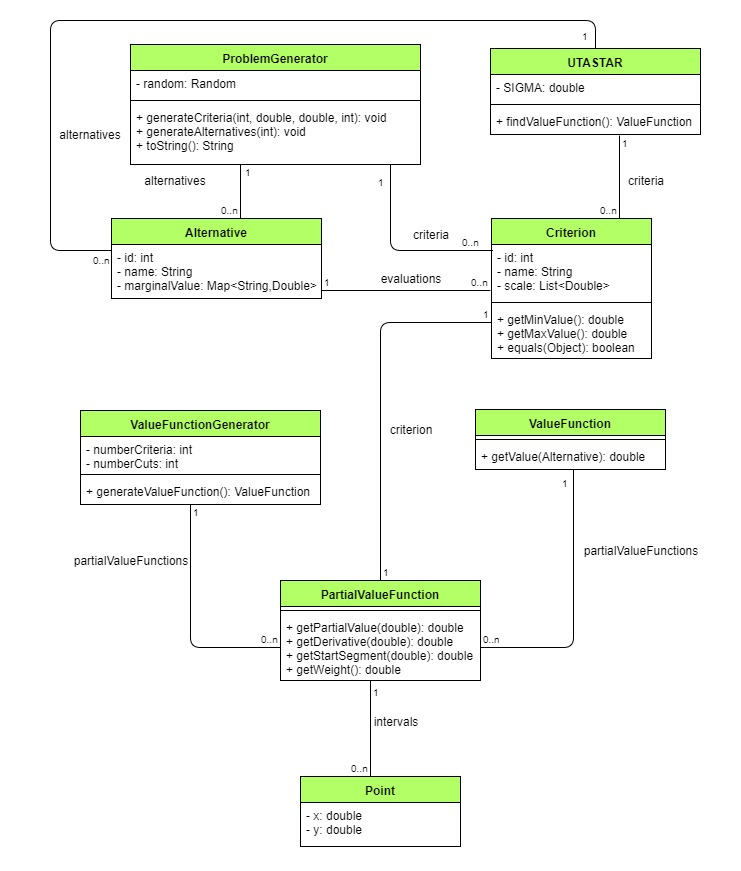
\includegraphics[width=17cm,height=17cm,keepaspectratio]{diagram-uml.png}
	\caption{Class Diagram}
\end{figure}
Other than the external libraries used in the resolution of a LP, no library is needed. \\

\subsubsection{Maven}
We figured out that we need to configure our project in Maven. Maven has been created to make a standard way to build a project and a way to share JAR files through many projects. Figuring out dependencies for small projects is not hard. But once the dependencies expand it will get out of hand. \\

Since we wanted to create an open source project, following the standards conventions was a must which led us to the use of Maven. Another plus of using Maven is that it provides a quality project information. \\

I personally prefer using the IDE Eclipse Luna to code in Java and I am currently using the version Luna 4.4.2 . So with Maven this won't be a big deal for people who don't use Eclipse, they can use NetBeans or IDEA or any other IDE that supports Maven.  \\

\underline{Configuration of Maven: }
\begin{itemize}
\item groupId: io.github.oliviercailloux
\item artifactId: uta-calculator
\end{itemize}

\subsection{Functionalities}
The following list represent the functionalities of the program I worked on:
\begin{itemize}
\item Program your own decision problem
\item Generate a random decision problem
\item Solve the decision problem by using UTASTAR algorithm
\item Elaborate a ValueFunction from a decision problem
\item Generate a ValueFunction
\item Available as open source
\end{itemize}
 
\subsection{Utils}
To make some function  more generic we created a package called utils, where we can find 2 java classes: 
\begin{itemize}
\item NumbersGenerator
\item ScaleGenerator
\end{itemize}

\subsubsection{NumbersGenerator}
The goal of this util class is to generate decimals numbers that have a certain sum. For example, If you want to create 3 numbers that have the sum of 1. \\
To make this possible, the class NumbersGenerator has the method generate that takes the following as parameters: 
\begin{enumerate}
\item counter (int)
\item targetSum (double)
\end{enumerate} 
The parameter counter represent the counter of numbers we want to generate, and the parameter targetSum represent the target sum we want. \\
You can specify the Random value in case you want to have the same result when doing testing. \\
This method will return a List of number of type double. 


\subsubsection{ScaleGenerator}
The goal of this util class is to generate scale for a criterion, where the interval $[ minValue, maxValue]$ is cut into equal intervals. For example, If you want the scale of criterion that have 10 as minimum value, 20 as maximum value and with 4 cuts, the function should return the following list: $[10.0, 13.333, 16.667, 20.0]$.\\
To make this possible, the class ScaleGenerator has the method generate that takes the following as parameters: 
\begin{enumerate}
\item minValue (double)
\item maxValue (double)
\item cuts (int)
\end{enumerate} 
The parameter minValue represent the minimum value of a criterion, the parameter maxValue represent the maximum value of a criterion and the parameter cuts represent the numbers of cuts you want to cuts the interval.  \\
This method will return a List of number of type double. 

\subsection{Simulation and Comparison}
TODO: To be made after the remarks of the program.

\subsection{Future Improvements}
This program has been done during the 3 month internship. Definitely it didn't take 3 month to make this program, but to been able to make such a program I had to make a research and learn about the UTA method. Basically we had to some cuts in order of complexity and compromise in some categories to make the implementation easier. And since the program will be available as an open source on GitHub, it has the potential to grow with some improvements. The following list is some of the improvements that could be made:\\
\begin{enumerate}
\item In the current version of the program, the criterion evaluation has a minimum value and maximum value, so the evaluation of a action is made in the range $[minValue, maxValue]$ with minValue being the least preferred criterion and maxValue the most preferred. But what if we want to represent a criterion that has maxValue as the least preferred criterion and minValue as the most preferred, like the criterion price. In the current version, this won't be possible. 
\item In our program, a criterion has a minimum value and maximum value, but what if the criterion is not a quantitative item, not evaluated in numbers. For example, let's say we want to evaluate the comfort, we can have the following values: 0, +, ++, +++ or not comfortable, basic, comfortable, very comfortable. So as an improvement we can expect to be able to design all of the criterion possible.  
\end{enumerate} 

TODO: To be continued...

\chapter{Conclusion}
\section{Difficulties encountered}
\section{Acquired Skills }


TODO: To be made this week...

\begin{thebibliography}{9}
\addcontentsline{toc}{chapter}{Bibliography}
\bibitem{multiple-criteria-decision-analysis} GRECO S., EHRGOTT M., RUI FIGUEIRA J., 2004, \textit{Multiple Criteria Decision Analysis}
\bibitem{cahier-lamsade-24} SISKOS J., 1979, \textit{Cahier du LAMSADE n24 : Les programmes UTA}
\bibitem{cahier-lamsade-49} SISKOS J., YANNACOPOULOS D., 1982, \textit{Cahier du LAMSADE n49 : Amélioration de la méthode UTA par introduction d’une double fonction d’erreurs}
\bibitem{these-hammami} HAMMAMI A., 2003, \textit{Thèse : Modélisation technico-économique d’une chaîne logistique dans une entreprise reseau}
\bibitem{study-stock-ranking} LUO H., SUN Z., 2014, \textit{A study on Stock Ranking and Selection Strategy Based on UTA Method under the Condition of Inconsistence}
\bibitem{multicriteria-decision-aid-methodology} ZOPOUNIDIS C., DOUMPOS M., 1997, \textit{A multicriteria decision aid methodology for the assessment of country risk}
\bibitem{development-utastar-method-fuzzy} EHSANIFAR M., ESHLAGHI A., KERAMATI M., NAZEMI J., 2013, \textit{The Development of UTASTAR Method in Fuzzy Environment for Supplier Selection}
\bibitem{application-methode-uta} SISKOS J., 1983, \textit{Application de la méthode UTA à un problème de sélection de points de vente mettant en jeu des critères multiples}
\end{thebibliography}

\listoffigures
\addcontentsline{toc}{chapter}{Table of figures}

\begin{appendices}

\selectlanguage{french}
\chapter{Compte Rendus avec M. Cailloux}
\section{CR1 - 15 juin 2017}
\textbf{15 juin 2017} / 15:00 / Université Paris Dauphine \\

\underline{Participants} \\

Olivier Cailloux, Elie Daher\\

\underline{Déroulement de la réunion}\\
\begin{itemize}
	\item Explication du plan du stage
	\item J’ai présenté les tâches effectuées
	\item J’avais quelques questions sur la méthode UTA et plus précisément sur un exemple “A Numerical Example” du chapitre 9 : ”UTA Method” du livre : “Multiple Criteria Decision Analysis”
	\item Présentation des tâches à effectuer\\
\end{itemize}

\underline{Les tâches à faire} \\
\begin{itemize}
	\item Créer un repository sur github
	\item Ecrire un résumé sur la méthode UTA en utilisant LaTeX
	\item En parallèle, effectuer des recherches sur des littératures existantes\\
\end{itemize}

\underline{Pièces jointes} \\
\begin{itemize}
	\item First iteration : document présenté par M. Cailloux qui contient le plan de la première itération\\
\end{itemize}

La réunion a été levée à 15:30\\

La prochaine réunion est prévue pour le mercredi 21 juin 2017 à 14:00


\newpage
\section{CR2 - 21 juin 2017}
\textbf{21 juin 2017} / 14:00 / Université Paris Dauphine \\

\underline{Participants} \\

Olivier Cailloux, Elie Daher\\

\underline{Déroulement de la réunion} \\
\begin{itemize}
	\item Présentation du travail effectué
	\item Résolution du projet java sur le programme linéaire\\
\end{itemize}

\underline{Les tâches à faire} \\
\begin{itemize}
	\item Rendre le document plus détaillé et développé
	\item Rendre le document plus compréhensible pour les lecteurs qui n’ont pas un context décisionnel
	\item Fixer le programme linear programming sur Java\\
\end{itemize}

La réunion a été levée à 14:40\\

La prochaine réunion est prévue pour le mercredi 28 juin 2017 à 11:00
\newpage
\section{CR3 - 28 juin 2017}
\textbf{28 juin 2017} / 11:00 / Université Paris Dauphine \\

\underline{Participants} \\

Olivier Cailloux, Elie Daher\\

\underline{Déroulement de la réunion}\\
\begin{itemize}
	\item Présentation du travail effectué
	\item Citer les remarques et les modifications à réaliser sur le document summary-uta et sur le repository de github (enlever le folder qui contient les *.class)
	\item Présentation du travail à effectuer pour la semaine prochaine\\
\end{itemize}

\underline{Les tâches à faire} \\
\begin{itemize}
	\item Corriger les remarques sur le document
	\item Développer $v^R$ et $v^T$
	\item Effectuer une recherche sur les littératures similaires déjà réalisées\\
\end{itemize}

La réunion a été levée à 11:30\\

La prochaine réunion est prévue pour le mercredi 5 juillet 2017 à 10:00

\newpage
\section{CR4 - 18 juillet 2017}
\textbf{18 juillet 2017} / 10:00 / Université Paris Dauphine \\

\underline{Participants} \\

Olivier Cailloux, Elie Daher\\

\underline{Déroulement de la réunion}\\
\begin{itemize}
	\item Présentation du travail effectué
	\item Explication de la fusion entre le projet Alternative-Criteria et UTA
	\item Apprendre comment télécharger des littératures à partir du site de la BU de Dauphine\\
\end{itemize}

\underline{Les tâches à faire} \\
\begin{itemize}
	\item Elaborer un document qui regroupe tout le travail effectué
	\item S’approfondir dans la recherche des littératures
	\item Fixer la méthode GenerateNumbers\\
\end{itemize}

La réunion a été levée à 10:45\\

La prochaine réunion est prévue pour le mardi 25 juillet 2017 à 10:00

\newpage
\section{CR5 - 25 juillet 2017}
\textbf{25 juillet 2017} / 10:00 / Université Paris Dauphine \\

\underline{Participants} \\

Olivier Cailloux, Elie Daher\\

\underline{Déroulement de la réunion}\\
\begin{itemize}
	\item Présentation du travail effectué
	\item Explication des modifications à faire dans le programme UTA
	\item Explication des modification à effectuer dans le document report\\
\end{itemize}

\underline{Les tâches à faire} \\
\begin{itemize}
	\item Ajouter les annexes des littérature dans le document
	\item Définir l’objectif de la méthode UTA dans le document
	\item Etablir les modifications sur le programme UTA
	\item Elaborer des résumés pour les articles trouvés\\
\end{itemize}

La réunion a été levée à 11:15\\

La prochaine réunion est prévue pour le lundi 31 juillet 2017 à 10:00

\newpage
\section{CR6 - 31 juillet 2017}
\textbf{31 juillet 2017} / 10:00 / Café Lumière - Hôtel Scribe\\

\underline{Participants} \\

Olivier Cailloux, Elie Daher\\

\underline{Déroulement de la réunion}\\
\begin{itemize}
	\item Présentation du travail effectué
	\item Refaire l’architecture du programme
	\item Présenter les modifications à faire\\
\end{itemize}

\underline{Les tâches à faire} \\
\begin{itemize}
	\item Elaborer des petits résumés pour les articles trouvés
	\item Compléter le rapport final
	\item Effectuer les modifications sur le programme\\
\end{itemize}

La réunion a été levée à 11:15\\

\chapter{Example of UTASTAR - Analyzing the choice of transportation}
A DM wants to analyse the choice of transportation. The DM is interstered in the following criteria 
\begin{enumerate}
\item price
\item time (min)
\item comfort (possibility to have a seat)
\end{enumerate}\leavevmode
The evaluation of the previous criteria is presented in the following table: 
\begin{center}
\begin{tabular}{ |c|c|c|c|c| } 
\hline
Means of transportation & Price & Time & Comfort & Ranking of the DM \\
\hline
RER & 3 & 10 & + & 1 \\
METRO (1) & 4 & 20 & ++ & 2 \\
METRO (2) & 2 & 20 & 0 & 2 \\
BUS & 6 & 40 & 0 & 3 \\
TAXI & 30 & 30 & +++ & 4 \\
\hline
\end{tabular}
\end{center}
DM's preferences: $ RER \succ  Metro1 \approx Metro2  \succ  Bus \succ  Taxi$\\
\newpage
First of all, we should specify the scale \footnote{the interval $[g_{i*}, g_{i}^{*}]$ is cut into equal intervals} for each criteria.
\begin{itemize}
\item Price  $\quad \rightarrow \quad [30, 16, 2]$
\item Time  $\quad \rightarrow \quad [40, 30, 20, 10]$
\item Comfort  $\quad \rightarrow \quad [0, +, ++, +++]$
\end{itemize}
According to this formula: $v(g(a)) = \sum_{i=1}^{n} v_i (g_i (a))$ , the value of each alternative may be written: 
\begin{itemize}
\item $v[g(RER)]= 0.07  v_1 (16) + 0.93 v_1(2) + v_2(10) + v_3(+)$
\item $v[g(METRO1)]= 0.14 v_1 (16) + 0.86 v_1(2) + v_2(20) + v_3(++)$
\item $v[g(METRO2)]= v_1 (2) + v_2(20) + v_3(0) =  v_1 (2) + v_2(20) $
\item $v[g(BUS)]= 0.29  v_1 (16) + 0.71 v_1(2) + v_2(40) + v_3(0) = 0.29 v_1 (16) + 0.71 v_1(2)$
\item $v[g(TAXI)]= v_1 (30) + v_2(30) + v_3(+++) = v_2(30) + v_3(+++)$
\end{itemize}
We have that $v_1(30) = v_2(40) = v_3(0) = 0$. \\
Since the marginal value $v_i(g_i)$ can be expressed in terms of variables $w_{ij}$: $v_i(g_i^{j}) = \sum _{t=1}^{j-1} w_{it}$ , the value of each alternative can be written: 
\begin{itemize}
\item $v[g(RER)]= w_{11} + 0.93 w_{12} + w_{21} + w_{22} + w_{23} + w_{31}$
\item $v[g(METRO1)]=w_{11} + 0.86 w_{12} + w_{21} + w_{22} + w_{31} + w_{32}$
\item $v[g(METRO2)]= w_{11} + w_{12} + w_{21} + w_{22} $
\item $v[g(BUS)]= w_{11} + 0.71 w_{12}$
\item $v[g(TAXI)]= w_{21} + w_{31} + w_{32} + w_{33}$
\end{itemize}
For each pair of consecutive alternatives, we express the difference between them: 
\begin{itemize}
\item $\Delta (RER, METRO1) = 0.07 w_{12} + w_{23} - w_{32} \geq \delta$
\item $\Delta (METRO1, METRO2) = -0.14 w_{12} + w_{31} + w_{32}  = 0$
\item $\Delta (METRO2, BUS) = 0.29 w_{12} + w_{21} + w_{22} \geq \delta$
\item $\Delta (BUS, TAXI) = w_{11} + 0.71w_{12} - w_{21} - w_{31} - w_{32} - w_{33} \geq \delta$
\end{itemize}
Having $\delta = 0.05$, we can solve the following LP:\\

Objective:  
\begin{equation}
	Minimize \quad \sum_{a \in A} \sigma _{a}^{+} + \sigma _{a}^{-}
\end{equation}

Subject to: \\
\begin{equation}
	\begin{cases}
		0.07 w_{12} + w_{23} - w_{32}  -\sigma _{RER}^{+} +\sigma _{RER}^{-} +\sigma _{METRO1}^{+} - \sigma _{METRO1}^{-}\geq \delta\\
		-0.14 w_{12} + w_{31} + w_{32}  -\sigma _{METRO1}^{+} +\sigma _{METRO1}^{-} +\sigma _{METRO2}^{+} - \sigma _{METRO2}^{-} = 0  \\
		 0.29 w_{12} + w_{21} + w_{22}  -\sigma _{METRO2}^{+} +\sigma _{METRO2}^{-} +\sigma _{BUS}^{+} - \sigma _{BUS}^{-} \geq \delta\\
		w_{11} + 0.71w_{12} - w_{21} - w_{31} - w_{32} - w_{33} -\sigma _{BUS}^{+} +\sigma _{BUS}^{-} +\sigma _{TAXI}^{+} - \sigma _{TAXI}^{-} \geq \delta\\
		w_{11} + w_{12} + w_{21} + w_{22} + w_{23} + w_{31} + w_{32} + w_{33} = 1\\

	\end{cases}
\end{equation}
So by using the com.google.ortools library, we can solve the Linear Program above with $\sigma = 0.05$. This Linear Program solution is coded in Java class ChoiceTransportation.\\
By executing the class ChoiceTransportation, you will have the following result: \\

An optimal solution is $w_{11} = 0.5$, $w_{22} = 0.05$, $w_{23} = 0.05$, $w_{33} = 0.4$ with $\sum_{a \in A} \sigma _{a}^{+} + \sigma _{a}^{-} = 0$. The utilities found for each alternative are as follows: \\ 
\begin{itemize}
\item $v(g(RER)) = 0.6$
\item $v(g(METRO1)) = 0.55$
\item $v(g(METRO2)) = 0.55$
\item $v(g(BUS)) = 0.5$
\item $v(g(TAXI)) = 0.4 $
\end{itemize}
Those utilities are consistent with the DM's preference ranking. \\

\chapter{Literature found during research}
\section{Literature used in the documentation}
\begin{itemize}
\item Multiple Criteria Decision Analysis - Salvatore Greco, Matthias Ehrgott, Jose Rui Figueira, 2004
\item Cahier du LAMSADE n24 : Les programmes UTA - J. Siskos, Octobre 1979
\item Cahier du LAMSADE n49 : Amélioration de la méthode UTA par introduction d’une double fonction d’erreurs - J.Siskos, D. Yannacopoulos, octobre 1983
\item Thèse : Modélisation technico-économique d’une chaîne logistique dans une entreprise reseau - Abdelkader Hammami, 2003
\item Assessing a set of additive utility functions for multicriteria decision-making, the UTA method
\item Assessing non-additive utility for multicriteria decision aid
\item Comparative analysis of UTA multicriteria methods
\item Preference disaggregation: 20 years of MCDA experience
\end{itemize}

\section{Useful literature}
\begin{itemize}
\item On the expressiveness of the additive value function and the Choquet integral models
\item ACUTA: A novel method for eliciting additive value functions on the basis of holistic preference statements
\item Stewart - Robustness of Additive Value Function Methods in MCDM (1996)
\item La Conception et l’implementation d’un outil d’aide a la decision multicriteres integrant les concepts de la gestion des connaissances et du cycle de vie: application de la chaine d’approvisionnement humanitaire
\item A study on Stock Ranking and Selection Strategy Based on UTA Method under the Condition of Inconsistence - Hong-chen Luo, Zhao-xu Sun, aout 2014
\item The Development of UTASTAR Method in Fuzzy Environment for Supplier Selection
\item A multicriteria decision aid methodology for the assessment of country risk
\item Application de la méthode UTA à un problème de sélection de points de vente mettant en jeu des critères multiples
\end{itemize}

\end{appendices}
\end{document}